\section{Methodology and Implementation}

	\subsection{Research Strategy and Approach}
	\noindent Before receiving the dataset, I have conducted an exhaustive investigation of the clinical landscape surrounding hypoglycaemia as a health condition, including studying the situations in which it commonly occurs, both in hospital settings as well as in public or everyday life. I have scrutinized a plethora of factors contributing to hypoglycaemia, including associated medicines (even conflicting medications), at-risk patient profiles, habits and lifestyles, dosing errors (both excessive as well as insufficient (\textit{insulin})), missed meals and even alcohol consumption. This has allowed me to better assess the quality of the incoming dataset and the relevance of its features. Upon requesting additional information regarding current patient medication and alcohol intake as it was not provided originally, GSTT advised that this data is unavailable because of its inconsistent self-reported nature and due to restrictions under their information governance policy that permits access to only the data deemed necessary for the project's scope.

	\vspace{10pt}
	\noindent After receiving the data, I have thoroughly preprocessed it to ensure it was suitable for meaningful analysis. This included addressing data type mismatches, deriving variables to aid in visualisation and understanding, and performing necessary imputations using appropriate methods. Duplicate and missing records were handled, categorical variables were encoded to make them compatible for predictive modelling, data validity and consistency checks were enacted to confirm that values were in expected ranges (for e.g. the glucose value field), normalization was carried out where necessary. These steps were necessary to lay a strong foundation for the subsequent application of statistical tests and machine learning models. The full preprocessing workflow is depicted in \autoref{fig:datapreprocessingwf} below. \
	
	\vspace{10pt}
	\noindent Following this, my focus was on exploratory data analysis to spot any anomalies or patterns near the surface. After devising research questions around the dataset, I have generated a collection of plots through Python's widely used seaborn library that I describe in detail in \hyperref[sec:mainResults]{the main results section}, which shed light on the prevalence of hypoglycaemia across various different scenarios. Special attention was paid to drawing comparisons between hypoglycaemic and non hypoglycaemic patients, in alignment with GSTT's interests that they had clarified in the project's early stages.

	\begin{figure}[H]
		\centering
		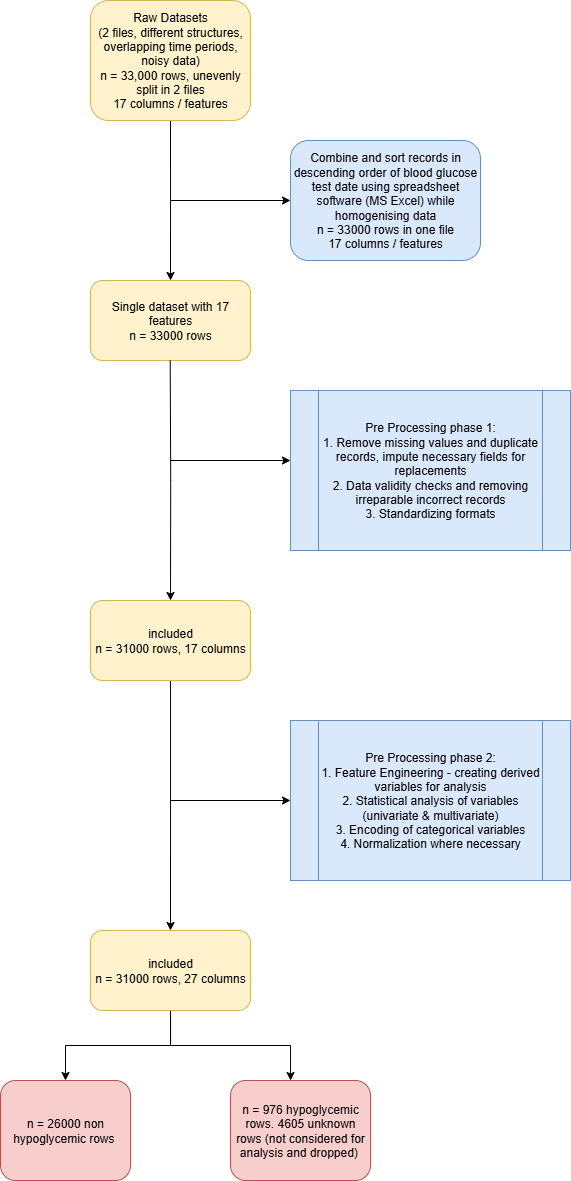
\includegraphics[height=8in]{figures/dataPreprocessingWf.png}
		\caption{Data preprocessing workflow}
		\label{fig:datapreprocessingwf}
	\end{figure}

	\subsection{Dealing With Imbalanced Data}
	augmentation / sampling

	\subsection{Machine Learning Theories}
	Decision tree
	random forest 
	grid search cv 
	conditional sampling 
	xgboost

	% It presents and justifies the methodology used to deal with the problem and describes in detail the implementation procedures. The background theory presented in the previous chapter can be recalled to support the proposed implementation. The originality, novelty and contribution are to be demonstrated with the discussion of the strengths and limitations.